% BHU PYQ -- Professional Exam Template
\documentclass[11pt,a4paper]{article}

\usepackage[a4paper,top=2.5cm,bottom=2.5cm,left=2.8cm,right=2.8cm,headheight=14pt]{geometry}
\usepackage{amsmath,amssymb}
\usepackage[T1]{fontenc}
\usepackage[utf8]{inputenc}
\usepackage{lmodern}
\usepackage{microtype}
\usepackage{fancyhdr}
\usepackage{enumitem}
\usepackage{hyperref}
\usepackage{lastpage}
\usepackage{parskip}
\usepackage{tikz}
\usetikzlibrary{arrows.meta,shapes,positioning}

\hypersetup{colorlinks=true,urlcolor=black,linkcolor=black,
  pdftitle={B.Sc. (Hons.) Zoology Sem-IV ZOB-401 -- BHU PYQ}}

\pagestyle{fancy}
\fancyhf{}
\renewcommand{\headrulewidth}{0.4pt}
\renewcommand{\footrulewidth}{0.4pt}
\fancyhead[L]{\small   \textit{Banaras Hindu University}}
\fancyhead[R]{\small   \textit{Zoology Paper: ZOB-401}}
\fancyfoot[C]{\small Page  \thepage\ of \pageref{LastPage}}


\newlist{parts}{enumerate}{2}
\setlist[parts,1]{label=(\alph*),leftmargin=*,itemsep=4pt,topsep=3pt}
\setlist[parts,2]{label=(\roman*),leftmargin=*,itemsep=2pt,topsep=2pt}

\newcommand{\pts}[1]{\hfill   \textit{[#1]}}


\begin{document}


\begin{center}
  {\large\bfseries BANARAS HINDU UNIVERSITY}\\[2pt]
  {\normalsize B.Sc. (Hons.) Semester IV Examination, 2022-23}\\[6pt]
  \rule{0.8\linewidth}{0.5pt}\\[6pt]
  {\large\bfseries Zoology}\\[4pt]
  {\large\bfseries Paper: ZOB-401 --- Fundamental Endocrinology and Economic Zoology}\\[4pt]
  {\normalsize Time: Three hours \hfill Full Marks: 70}
\end{center}

\rule{\linewidth}{0.4pt}

\smallskip



\noindent   \textit{Note: Answer three questions from Section-A and three questions from Section-B. Question No. 1 in both sections is compulsory. Use a separate answer book for each section. The figures in the right-hand margin indicate marks.}

\bigskip

\begin{center}
   \textbf{SECTION -- A} \\
   \textbf{(Fundamental Endocrinology) (Marks: 35)}
\end{center}

\medskip


\noindent   \textbf{Question 1.} Answer the following parts:

\begin{parts}
  \item Define the following terms:\pts{$1  \times 3 = 3$}
  
\begin{parts}
    \item Bursicon
    \item Cretinism
    \item Relaxin
  \end{parts}

  \item Differentiate between the following:\pts{$2  \times 2 = 4$}
  
\begin{parts}
    \item Negative and Positive feedback mechanisms
    \item Sertoli cells and Leydig cells
  \end{parts}

  \item Justify giving reasons whether the following statements are True or False:\pts{$2  \times 2 = 4$}
  
\begin{parts}
    \item Environmental factors affect thyroid hormone secretions.
    \item Glucagon is a hypoglycemic hormone.
  \end{parts}
\end{parts}

\medskip


\noindent   \textbf{Question 2.} Answer the following parts:

\begin{parts}
  \item Define hormones and classify them according to their structural and functional similarities.\pts{6}
  \item How does the pineal gland coordinate daily rhythms? Explain with the help of a flowchart.\pts{6}

  
\begin{center}
  
\begin{tikzpicture}[scale=1.0, >=Stealth, every node/.style={font=\small, draw, rounded corners, fill=blue!5, align=center, minimum height=0.8cm}]
    % Flowchart Nodes
    
ode (light) at (0,4) {Environmental Light / Dark Cycle};
    
ode (retina) at (0,2.5) {Retina (Photoreceptors)};
    
ode (scn) at (0,1) {Suprachiasmatic Nucleus (SCN)\\ (Circadian Pacemaker)};
    
ode (scg) at (0,-0.5) {Superior Cervical Ganglion (SCG)};
    
ode (pineal) at (0,-2) {Pineal Gland};
    
ode (melatonin) at (0,-3.5) {Melatonin Secretion\\ (High in Dark, Low in Light)};
    
ode (rhythms) at (0,-5) [fill=green!10] {Regulation of Circadian Rhythms\\ (Sleep-wake cycle, body temp)};
    
    % Connective Arrows
    \draw[->, thick] (light) -- (retina);
    \draw[->, thick] (retina) -- node[draw=none, fill=none, right] {Retinohypothalamic Tract} (scn);
    \draw[->, thick] (scn) -- (scg);
    \draw[->, thick] (scg) -- node[draw=none, fill=none, right] {Sympathetic pathway} (pineal);
    \draw[->, thick] (pineal) -- (melatonin);
    \draw[->, thick] (melatonin) -- (rhythms);
  \end{tikzpicture}
  \end{center}
\end{parts}

\pagebreak
\medskip


\noindent   \textbf{Question 3.} Answer the following parts:

\begin{parts}
  \item Draw a neat and well-labeled diagram of the adrenal gland. Also mention the biological actions of all the adrenocortical hormones.\pts{8}

  
\begin{center}
  
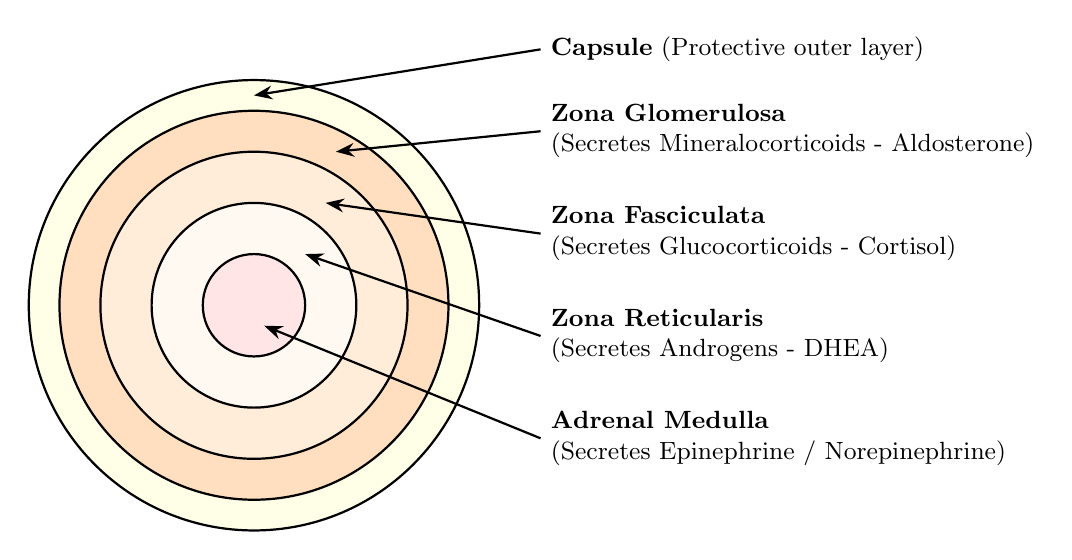
\begin{tikzpicture}[scale=1.3, >=Stealth, every node/.style={font=\small}]
    % Concentric zones of adrenal gland
    \draw[thick, fill=yellow!10!white] (0,0) circle (2.2); % Capsule / Outer border
    \draw[thick, fill=orange!25!white] (0,0) circle (1.9); % Zona Glomerulosa
    \draw[thick, fill=orange!15!white] (0,0) circle (1.5); % Zona Fasciculata
    \draw[thick, fill=orange!5!white] (0,0) circle (1.0);  % Zona Reticularis
    \draw[thick, fill=red!10!white] (0,0) circle (0.5);    % Medulla

    % Medulla text
    
ode at (0,0) {   \textbf{Medulla}};
    
    % Labels and Callout lines
    \draw[<-, thick] (0, 2.05) -- (2.8, 2.5) node[right, align=left] {   \textbf{Capsule} (Protective outer layer)};
    \draw[<-, thick] (0.8, 1.5) -- (2.8, 1.7) node[right, align=left] {   \textbf{Zona Glomerulosa} \\ (Secretes Mineralocorticoids - Aldosterone)};
    \draw[<-, thick] (0.7, 1.0) -- (2.8, 0.7) node[right, align=left] {   \textbf{Zona Fasciculata} \\ (Secretes Glucocorticoids - Cortisol)};
    \draw[<-, thick] (0.5, 0.5) -- (2.8, -0.3) node[right, align=left] {   \textbf{Zona Reticularis} \\ (Secretes Androgens - DHEA)};
    \draw[<-, thick] (0.1, -0.2) -- (2.8, -1.3) node[right, align=left] {   \textbf{Adrenal Medulla} \\ (Secretes Epinephrine / Norepinephrine)};
  \end{tikzpicture}
  \end{center}

  \item Describe the neurohypophysial hormone family.\pts{4}
\end{parts}

\medskip


\noindent   \textbf{Question 4.} Write short notes on any two of the following:\pts{$6  \times 2 = 12$}

\begin{parts}
  \item Calcium homeostasis
  
  
\begin{center}
  
\begin{tikzpicture}[scale=0.9, >=Stealth, every node/.style={font=\small, align=center}]
    % High/Low blood calcium levels loop
    
ode (normal) at (0,0) [draw, rounded corners, fill=gray!10] {   \textbf{Normal Blood $Ca^{2+}$ Level}\\ ($\approx 10 \text{ mg/dL}$)};
    
    % Low blood calcium pathway
    
ode (low) at (-3.5, 1.5) [draw, rounded corners, fill=red!5] {Low Blood $Ca^{2+}$};
    
ode (pth) at (-3.5, 3.2) [draw, rounded corners, fill=orange!5] {Parathyroid Gland\\ releases   \textbf{PTH}};
    
ode (pth-act) at (-3.5, 4.8) [draw, rounded corners, fill=orange!10] {Reabsorption from kidney\\ Ca release from bone\\ Absorption in intestine};
    
    % High blood calcium pathway
    
ode (high) at (3.5, 1.5) [draw, rounded corners, fill=blue!5] {High Blood $Ca^{2+}$};
    
ode (calcitonin) at (3.5, 3.2) [draw, rounded corners, fill=cyan!5] {Thyroid Gland\\ releases   \textbf{Calcitonin}};
    
ode (calc-act) at (3.5, 4.8) [draw, rounded corners, fill=cyan!10] {Deposition in bones\\ Excretion in kidney};

    % Connections
    \draw[->, thick] (normal) to[out=135, in=270] (low);
    \draw[->, thick] (low) -- (pth);
    \draw[->, thick] (pth) -- (pth-act);
    \draw[->, thick] (pth-act) to[out=0, in=90] (normal);
    
    \draw[->, thick] (normal) to[out=45, in=270] (high);
    \draw[->, thick] (high) -- (calcitonin);
    \draw[->, thick] (calcitonin) -- (calc-act);
    \draw[->, thick] (calc-act) to[out=180, in=90] (normal);
  \end{tikzpicture}
  \end{center}

  \item Graafian follicle
  \item Ecdysteroids
\end{parts}

\bigskip

\begin{center}
   \textbf{SECTION -- B} \\
   \textbf{(Economic Zoology) (Marks: 35)}
\end{center}

\medskip


\noindent   \textbf{Question 1.} Answer the following parts:

\begin{parts}
  \item Write whether the following statements are True or False. Justify your answers in 2-3 sentences each:\pts{$2  \times 3 = 6$}
  
\begin{parts}
    \item Female silk moths survive about 3 years.
    \item Male and female lac insects reside in similar shaped resin cells.
    \item Leghorn, Minorca and Ancona are good egg layers.
  \end{parts}
  
  \item Define the following terms:\pts{$1  \times 5 = 5$}
  
\begin{parts}
    \item Pullets
    \item Heifer
    \item Bee-economics
    \item Seed lac
    \item Waggle dance
  \end{parts}
\end{parts}

\medskip


\noindent   \textbf{Question 2.} Describe the steps of fish culture, mode of breeding and methods of fish preservation.\pts{12}

\medskip


\noindent   \textbf{Question 3.} Write an essay on milk and milk products.\pts{12}

\medskip


\noindent   \textbf{Question 4.} Answer the following parts:

\begin{parts}
  \item Write an essay on the diseases of silkworms.\pts{8}
  \item Write about the economic importance of honeybees.\pts{4}
\end{parts}

\vfill
\rule{\linewidth}{0.4pt}

\begin{center}\small
\href{https://bhu-exam.vercel.app/}{Click Here}\\[4pt]\href{https://me-aryan.vercel.app/}{Click Here}\\[4pt]\href{https://quashan-me.vercel.app/}{Click Here}
\end{center}

\end{document}
